Für die Umsetzung verschiedener höher liegender Strategien ist es wichtig den NAO mit Ball an neue Positionen zu manövrieren. Eine Dribbelfunktion, die so etwas leisten könnte war jedoch im Framework nie vorhanden oder wurde entfernt. So war eine Konstante \textit{MOVE\_WITH\_BALL} zwar in \texttt{magma.agent.behavior.IBehaviorConstants} vorhanden, ihr wurde jedoch keine Implementierung zugewiesen.\\
Deshalb wurde ein eigenes Behavior (\texttt{magma.robots.robofreunde.behavior.complex.DribbleWithBall})zu diesem Zweck entwickelt.

\subsubsection{Grundidee}
Da der Kick zum Entwicklungszeitpunkt der Dribbelfunktion nur sporadisch erfolgreich war, wurde als Grundlage das Laufen verwendet. Läuft der NAO gegen den Ball, so rollt dieser von ihm weg. Geschieht dies nun aus der richtigen Richtung, bewegen sich sowohl der Roboter als auch der Ball in die gewünschte Richtung. Aufgrund der geringeren Berührungsintensität am Ball, im Vergleich zum Kick, bleibt so auch die maximale Distanz zwischen diesem und dem NAO beim dribbeln kleiner.

\subsubsection{Positionierung}
Für die Positionierung zum Ball wird der relative Vektor von diesem zum Ziel berechnet und von dessen Position abgezogen. Die so berechnete Stelle liegt auf einer Linie mit dem Ball und dem Ziel. Erreicht der NAO diesen Ort, liegt der Ball genau zwischen ihm und dem gewünschten Ziel. In der Theorie schiebt der Roboter nun den Ball, während er sich auf das Ziel zu bewegt.

\subsubsection{Ball dribbeln}
Um zu verhindern, dass der NAO beim Versuch zu dribbeln den vor sich liegenden Ball als Hindernis erkennt, welchem er ausweichen soll, wurde ein neues Lauf-Behavoir (\texttt{magma.robots.robofreunde.behavior.complex.HulkToPosition}) vom bestehenden abgeleitet. Dieses ignoriert alle Hindernisse auf seinem Weg und bringt den NAO unsicher ans Ziel.

\subsubsection{Ausrichtung zum Ball}
Beim Bewegen zum gewünschten Ziel überprüft der NAO dabei ständig ob der Ball noch richtig liegt. Zu diesem Zweck wird ein Rechteck zwischen dem Ziel und der eigenen Position ausgespannt, dessen Breite kleiner ist als die des NAOs. Rollt der Ball nun über eine der Seitenlinien wird dies erkannt und eine Neupositionierung eingeleitet. Eine ungültige Seitenlinie wird im Debugger durch eine rote Färbung kenntlich gemacht, gültige sind grün.


\begin{lstlisting}[caption=Ausrichtung zum Ball, captionpos=b, label=lst:aligned-with-ball]
/**
 * Checks alignment with the ball via rectangle.
 * @param epsilon Allowed Distance from Ball to direct line.
 * @return True if the player is aligned with the ball.
 */
private boolean isAlignedWithBallReckt(double epsilon) {
    Vector3D leftPoint = getMyPosition().add(epsilon, new Vector3D(getAngleToPosition() + Math.toRadians(90), 0.0));
    Vector3D rightPoint = getMyPosition().add(epsilon, new Vector3D(getAngleToPosition() - Math.toRadians(90), 0.0));
    double leftAngleToBall = getBallPosition().subtract(leftPoint).getAlpha()
            - getMyPosition().subtract(leftPoint).getAlpha();
    double rightAngleToBall = getBallPosition().subtract(rightPoint).getAlpha()
            - getMyPosition().subtract(rightPoint).getAlpha();
    leftAngleToBall += leftAngleToBall < 0 ? 2* Math.PI : 0;
    rightAngleToBall += rightAngleToBall < 0 ? 2* Math.PI : 0;
    boolean isAlignedLeft = 0 < Math.toDegrees(leftAngleToBall) && Math.toDegrees(leftAngleToBall) < 90;
    boolean isAlignedRight = 270 < Math.toDegrees(rightAngleToBall) && Math.toDegrees(rightAngleToBall) < 360;
    if (!getDebugger().isHidden()) {
        getDebugger().drawLine(leftPoint
                , leftPoint.add(desiredBallPosition.subtract(getMyPosition()))
                , getValidationColor(isAlignedLeft));
        getDebugger().drawLine(rightPoint
                , rightPoint.add(desiredBallPosition.subtract(getMyPosition()))
                , getValidationColor(isAlignedRight));

    }
    return isAlignedLeft && isAlignedRight;
}
\end{lstlisting}

\subsubsection{Ausrichtung zum Ziel}
Da zwar der Ball im Rechteck liegen, der NAO aber verdreht zum Ziel stehen kann, wird auch diese Ausrichtung überprüft. Dabei der Winkel gemessen, der zwischen der aktuellen Ausrichtung des Bots und der Zielposition liegt. Ist dieser größer als ein zulässiger Maximalwert, wird eine Neupositionierung eingeleitet.\\
Befindet sich der NAO nahe am Ziel, ist eine größere Abweichung weniger schlimm, da schon kleine Änderungen im Ort große Auswirkungen auf den Winkel haben. Um diesem Umstand gerecht zu werden, wird der zulässige Maximalwert in Abhängigkeit zur Entfernung zum Ziel erhöht. Im Debugger werden die äußersten zulässigen Winkel durch Schenkelstücke dargestellt. Liegt das Ziel nicht innerhalb der Grenzen wechselt deren Farbe von Grün auf Rot.


\begin{lstlisting}[caption=Ausrichtung zum Ziel, captionpos=b, label=lst:facing-target]
/**
 * Checks whether the Nao is facing it's target.
 * @return True if the Nao is facing the target.
 */
private boolean isFacingTarget() {
    double validAngle = Math.toRadians(6.0) * getFuzzyMultiplier(desiredBallPosition);
    boolean isFacing = Math.abs(getAngleToPosition() - getPlayerAngle()) < validAngle;
    if (!getDebugger().isHidden()) {
        RoboVizColors color = getValidationColor(isFacing);
        getDebugger().drawLine(getMyPosition()
                , getMyPosition().add(new Vector3D(getPlayerAngle() - validAngle, 0.0)), color);
        getDebugger().drawLine(getMyPosition()
                , getMyPosition().add(new Vector3D(getPlayerAngle() + validAngle, 0.0)), color);
    }
    return isFacing;
}
\end{lstlisting}

\subsubsection{MetricBot}
Zur Bewertung des Optimierungsfortschritts wurde ein Decisionmaker implementiert, der einen gegebenen Parkour abdribbelt. Die benötigte Zeit gilt als zu minimierendes Kriterium. Im Laufe der Tests wurden so auch Schwächen einer Überprüfung der Ausrichtung zum Ball via Winkel aufgedeckt. Sie hatten die Implementierung der Funktion in ihrem aktuellen Zustand zur Folge.\\
In guten Versuchen liegt die benötigte Zeit für den Parkour mit einem Dribbeln des Balls nur circa ein Drittel höher als beim reinen Ablaufen ohne Ball.

\begin{figure}[H]
	\centering
	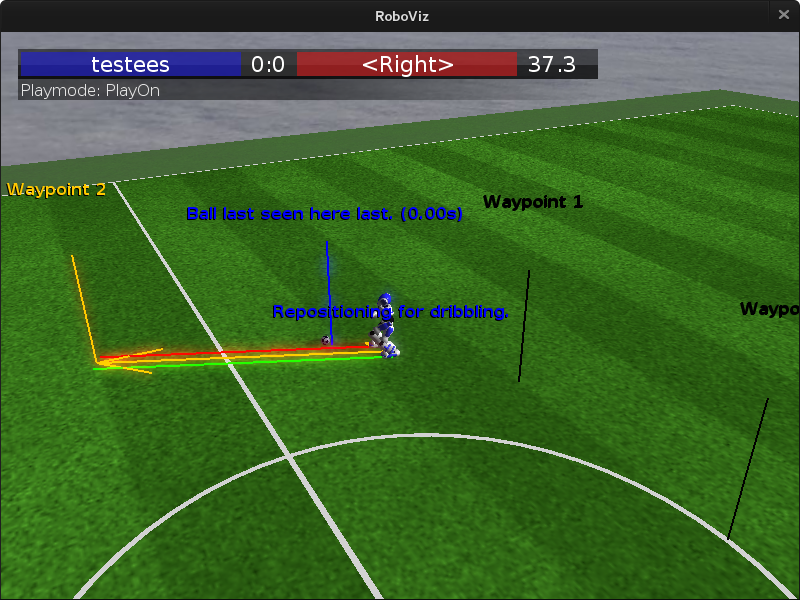
\includegraphics[width=\ScaleIfNeeded]{Grafiken/Dribble/DribbleRektReposition}
	\caption{Dribble Bot}
	\label{fig:dribblerekt}
\end{figure}